\documentclass{article}
\usepackage[utf8]{inputenc}
\usepackage[margin=1in]{geometry}
\usepackage{listings}
\usepackage{xcolor}
\usepackage{booktabs}
\usepackage{graphicx}

\definecolor{codegreen}{rgb}{0,0.6,0}
\definecolor{codegray}{rgb}{0.5,0.5,0.5}
\definecolor{codepurple}{rgb}{0.58,0,0.82}
\definecolor{backcolour}{rgb}{0.95,0.95,0.92}

\lstdefinestyle{mystyle}
{
	backgroundcolor=\color{backcolour},   
	commentstyle=\color{codegreen},
	keywordstyle=\color{magenta},
	numberstyle=\tiny\color{codegray},
	stringstyle=\color{codepurple},
	basicstyle=\ttfamily\footnotesize,
	breakatwhitespace=false,         
	breaklines=true,                 
	captionpos=b,                    
	keepspaces=true,                 
	numbers=left,                    
	numbersep=5pt,                  
	showspaces=false,                
	showstringspaces=false,
	showtabs=false,                  
	tabsize=2
}

\lstset{style=mystyle}
\begin{document}
\begin{titlepage} % Suppresses displaying the page number on the title page and the subsequent page counts as page 1
		
		\raggedleft\rule{1pt}{\textheight} % Vertical line
		\hspace{0.05\textwidth} % Whitespace between the vertical line and title page text
		\parbox[b]{0.75\textwidth}
		{ % Paragraph box for holding the title page text, adjust the width to move the title page left or right on the page
			
			{\Huge\bfseries MIT World Peace University \\[0.5\baselineskip] \ Python Programming}\\[2\baselineskip] % Title
			{\large\textit{Assignment 5}}\\[4\baselineskip] % Subtitle or further description
			{\Large\textsc{Naman Soni Roll No. 10}} % Author name, lower case for consistent small caps
			
			\vspace{0.5\textheight} % Whitespace between the title block and the publisher
		}
		
\end{titlepage}
	% \tableofcontents
	% \pagebreak
% \section{\textbf{Problem Statement}}
% To find largest of three numbers.
% \section{\textbf{Aim}}
% Write a python program to find largest of three numbers.
% \section{\textbf{Objectives}}
% To learn and implement different forms of if..else statement.
% \section{\textbf{Theory}}
% \subsection{\textit{Decision Making}}
% Following is the general form of a typical decision-making structure found in most of the
% programming languages-
% \begin{center}
% 	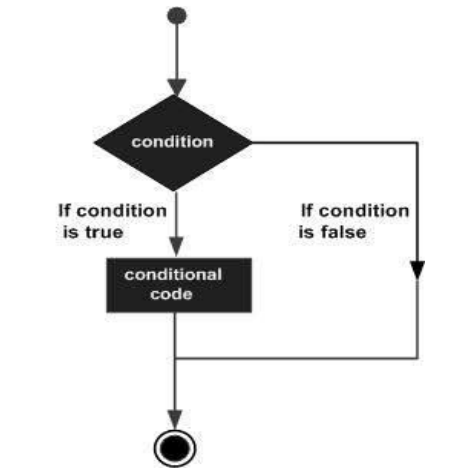
\includegraphics[0.5]{ass2.png}
% \end{center}
% Python programming language assumes any non-zero and non-null values as TRUE, and if it is either zero or null, then it is assumed as FALSE value.\\
% Python programming language provides following types of decision-making statements.

\end{document}